\documentclass[12pt]{beamer}
\usecolortheme{ietf93color}

\mode<presentation>
\title{IS-IS Point to Multipoint operation}
\subtitle{%
  \href{https://datatracker.ietf.org/doc/draft-lamparter-isis-p2mp/}{draft-lamparter-isis-p2mp-00}
}
\author{%
\href{mailto:chris@opensourcerouting.org}{Christian Franke $\cdot$ chris@opensourcerouting.org}\\%
\underline{\href{mailto:david@opensourcerouting.org}{David Lamparter $\cdot$ david@opensourcerouting.org}}%
}
\date{IETF 93, Prague, July 2015}
\begin{document}

\begin{frame}
  \titlepage
\end{frame}

\begin{frame}
  \frametitle{Starting problem}
  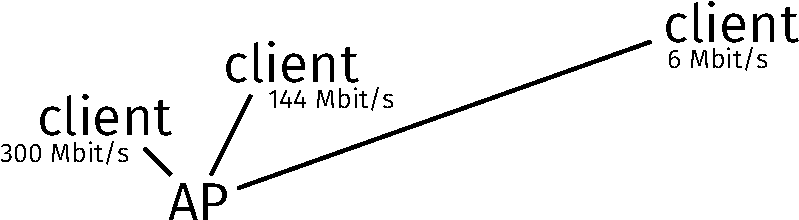
\includegraphics[scale=0.65,angle=0]{isis_93_wifitopo.pdf}%
  \vspace{5mm}
  \begin{itemize}
    \item 802.11 metrics vary wildly inside a broadcast domain
    \item all station to station packets relayed by AP
    \item slow and unreliable multicast
  \end{itemize}
\end{frame}

\begin{frame}
  \frametitle{Applicability check}
  Some problems can be worked around:
  \begin{itemize}
    \item 802.11v and 11aa add reliable multicast
    \item software can improve multicast TX rate
  \end{itemize}
  Some cannot:
  \begin{itemize}
    \item cost is a function of (sender,receiver) pair
  \end{itemize}
\end{frame}

\begin{frame}
  \frametitle{IS-IS approach}

  Use PtP on broadcast ala RFC 5309 (P2P over LAN), but support more than one adjacency.

  \vspace{5mm}
  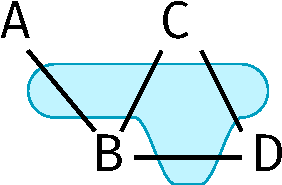
\includegraphics[scale=0.65,angle=0]{isis_93_p2mplink.pdf}%
  \vspace{5mm}

  \begin{itemize}
    \item need to demultiplex received packets, adjacencies will interfere with each other
    \item want some discovery protocol
  \end{itemize}
\end{frame}

\begin{frame}
  \frametitle{P2MP Adjacencies}

  Introducing "\underline{pseudocircuit}" as name for an individual (PtP) adjacency on a P2MP link.

  \vspace{5mm}

  Uses a separate new P2MP Hello PDU type:
  \begin{itemize}
    \item P2MP Hello w/o RFC5303 3-way Adj TLV for discovery
    \item P2MP Hello with RFC5303 3-way Adj TLV for adjacency maintenance
  \end{itemize}
\end{frame}

\begin{frame}
  \frametitle{Single router view}

  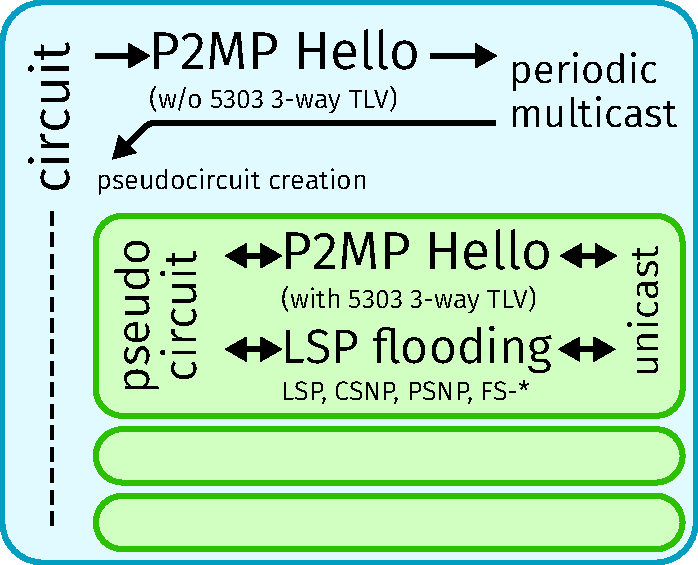
\includegraphics[scale=0.70,angle=0]{isis_93_p2mpmech.pdf}%
\end{frame}

\begin{frame}
  \frametitle{PDUs and TLVs}

  \begin{itemize}
    \item no new TLVs added by this draft
    \item packets demultiplexed by packet source address
    \item packets sent to neighbor's unicast destination address
  \end{itemize}
\end{frame}

\begin{frame}
  \frametitle{LSP / Flooding behavior}

  \begin{itemize}
    \item {\Large no change to PtP flooding mechanics}
    \item packets demultiplexed by packet source address
    \item packets sent to neighbor's unicast destination address
  \end{itemize}
\end{frame}

\begin{frame}
  \frametitle{Generated TLVs}

  \begin{itemize}
    \item {\Large P2MP is invisible to rest of IS-IS domain}
    \item SPF calculation sees a bunch of PtP links
    \item can be deployed on per-link basis
  \end{itemize}
\end{frame}

\begin{frame}
  \frametitle{Next steps}
  \begin{itemize}
    \item fixing TODOs in draft
    \item support multicast LSP/CSNP/PSNP on P2MP?
    \item feedback?
  \end{itemize}
\end{frame}

\end{document}
